\chapter{Context Survey}

Here I will review the existing software and literature on the different aspects of this project. 
I will briefly look at the psychological and gamification considerations around this topic to provide context, however the focus will be on the existing technologies.


\section{Opinion of First Contact?}
As this project has been undertaken in collaboration with the Exoplanet Research Society, it is worth briefly reviewing the literature on the target question - how would humans react to the discovery of alien life? There has been some research\cite{ReactionsToMessage, HowReactDiscovery, Fear} into this area, but it is certainly not extensive and very little of it is systematic. The topic is vast with many variations:
\begin{itemize}
    \item How has extra-terrestrial life been discovered?
    \item What is the nature of the life, is it intelligent?
    \item Is alien life on our doorstep, or far enough away that it could never reach or harm us?
\end{itemize}
Anne Smith and Christine Helling believe it could be beneficial to create a game capable of collecting this information, in order to reduce the burden on participants answering such an extensive library of questions and improve engagement. If this was possible it would have the potential to impact the way opinion data is collected across multiple faculties.

\section{Survey Gamification}
An emerging trend in modern business practice, gamification can be defined as `using game mechanics and game design elements to measure, influence and reward user behaviors.'~\cite{7804551}. 
There has been research into gamification as a tool to improve the quality of responses from and engagement with surveys. From this I aim to gain an awareness of the necessary considerations when implementing gamification.

As of yet, most experiments into survey gamification have only gone so far as to change the wording of survey questions, show questions alongside imagery or change the answer input mechanics.
My project represents a considerable departure from the standard survey format, with the goal being that the player could enjoy the game as a standalone experience. 
Because of this, there are many psychological considerations as to the validity of the results that can be gathered through this format. 
While investigating these issues is not my goal, I deemed it important to understand them, in an attempt to minimise any bias that my framework could impose onto players.

A 2011 paper found that while participants' enjoyment of the survey sees a great increase, gamification has three aspects which can affect the `character of the data'~\cite{GameExperiments}:
\begin{enumerate}
    \item Effects caused by changes to the question and how it is interpreted
    \item Effects caused by changing the attitude and mindset of respondents
    \item Effects caused by changes to the design and layout of question
\end{enumerate}
These considerations are targeted towards the low levels of gamification previously discussed, where the questions still have a fairly standard format. 
I do however believe that they are still applicable to my project. 

The design of my game adds context that persists between questions. 
A 2015 paper\cite{Olympic} states `Designers may also implement feedback loops, i.e., dynamics wherein user actions affect the overall state of gameplay. Feedback loops may visualize concepts such as a user’s progress, status, wealth, health, points, etc.'. 
This gives me confidence that adding a persistent context to the game is a valid design decision, which I believe relates to the first point above - `Effects caused by changes to the question and how it is interpreted'. This is because changing the context effectively changes the question, as people may respond differently under different circumstances. 

`Effects caused by changes to the design and layout of question' will also appear in my artifact - there must be some UI to interact with, and as such it is possible that this may affect the player's choices. I attempt to minimise this risk - ideally the only bias imposed should be from the game description itself.

Briana Brownell, Jared Cechanowicz, and Carl Gutwin summarise the state of research into survey gamification as follows:
`In most cases, their results show that the addition of these game elements increases the length and quantity of responses, and respondents typically prefer the gamified version to the standard survey version. However, their research does not compare the effectiveness of game elements in gamified surveys. They have also found that that some gamified survey designs can lead to compromised respondent data (Puleston \& Sleep, 2011).'~\cite{SurveyGamificationResearch}.
This indicates that there is promise in the notion of gamifying surveys - however, gamification can result in a reduction in the accuracy of the data collected. Depending on the extent to which the survey is abstracted from, precise details, both of the question and response, can be lost. Given this, gamification is likely best suited to situations in which the surveyors do not need precise answers.

\section{Similar Software}

\subsection{Datagame}
Datagame\cite{Datagame} offers services that allow researchers to create and publish gamified surveys. This is done through heavily game-influenced interfaces, such as word searches and decks of cards.

Datagame supplies the tools required to populate one of several template games with custom questions, and export this to an online format that can be played through many channels such as Facebook\cite{Facebook}. 

There are four game types available to customise. The one most similar to the kind I intend to create is referred to as a `Swiper' game. In this, the player draws cards from a virtual deck, each of which presents a yes/no question. The user swipes the card left or right, to answer yes or no respectively. Figure \ref{fig:datagame} shows this interface - it is fairly simple, with no standout features other than those added during admin configuration. Customisation allows the user to replace card backgrounds with an images, as well as change the colour of the text. Figure \ref{fig:dg_editor} shows an example of the game editing view in which the following aspects of the game can be edited:

\begin{itemize}
    \item Project title
    \item Title question
    \item List of cards
    \item Card name
    \item Card text/images
    \item Toggle card shuffling
    \item Game UI labels
    \item Background image
\end{itemize}

\begin{figure}[!h]
	\centering
	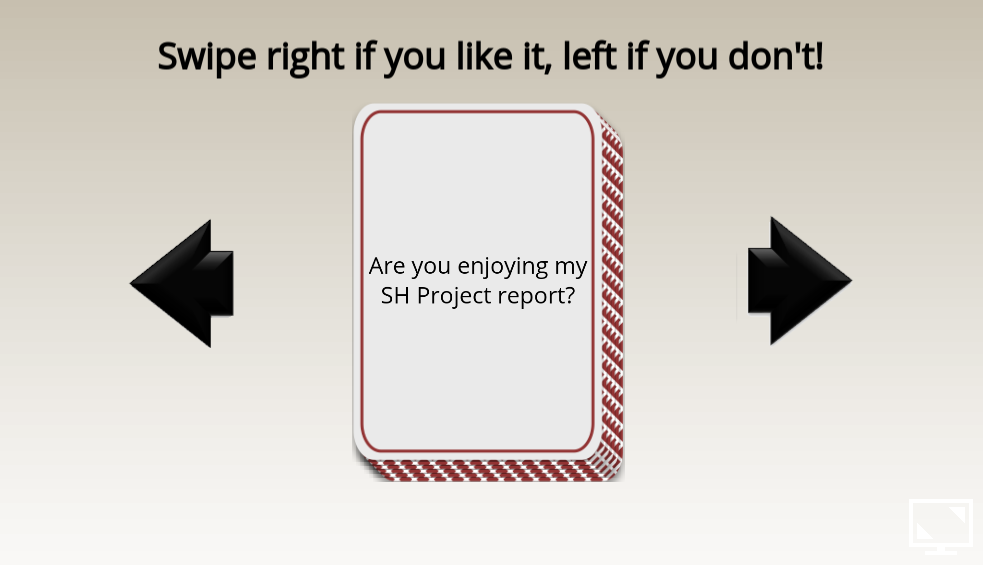
\includegraphics[width=1.0\textwidth]{./images/context/datagame.png}
	\caption{Example question in one of the Datagame\cite{Datagame} game types, which involves answering yes or no questions by swiping left or right.}
	\label{fig:datagame}
\end{figure}

\begin{figure}[!h]
	\centering
	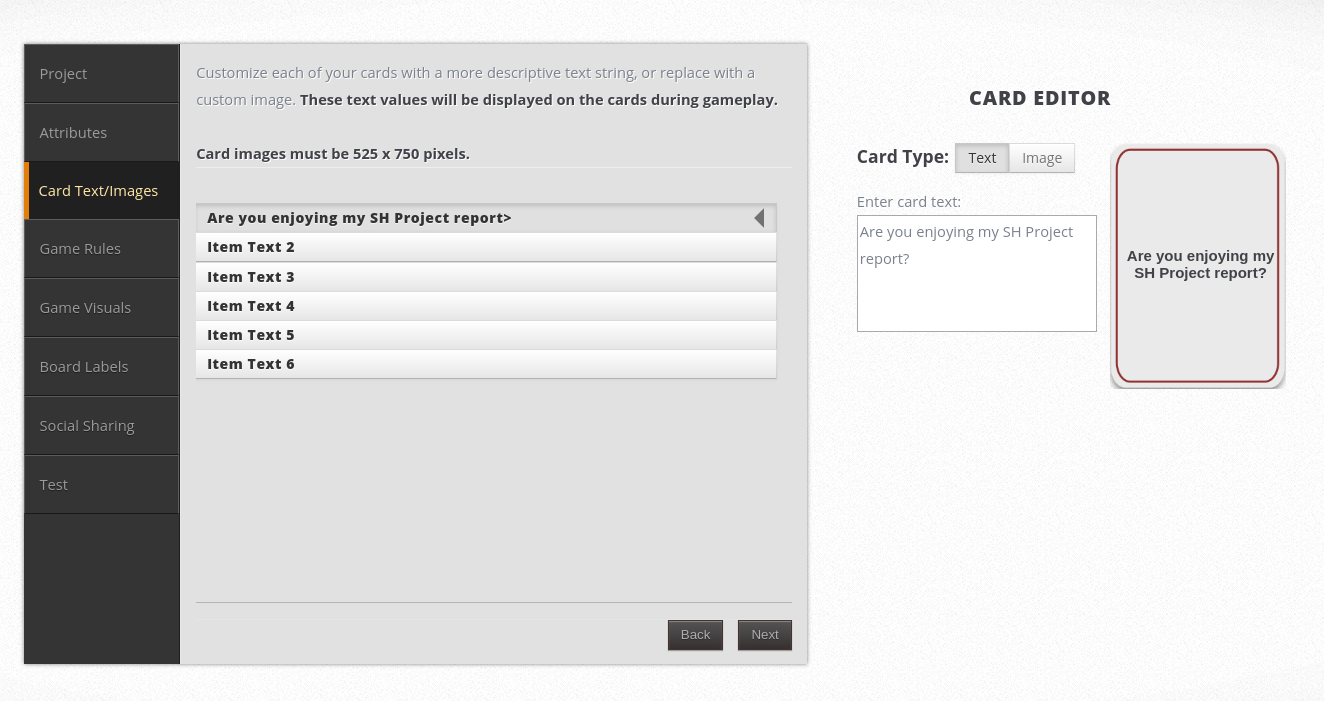
\includegraphics[width=1.0\textwidth]{./images/context/dg_editor.png}
	\caption{Process of editing the Datagame\cite{Datagame} game instance shown in figure \ref{fig:datagame}. }
	\label{fig:dg_editor}
\end{figure}

\subsection{Qualifio}
Qualifio\cite{Qualifio} offer a similar service. They provide more varied game formats than Datagame, but the presentation is less game-like. 

\subsection{Reigns}
When proposing the format of the artifact, I based my framework on an existing game, Reigns~\cite{Reigns}. 
In Reigns, the player takes the role of a medieval ruler, and makes binary decisions to solve problems their subjects approach them with. 
These decisions affect further scenarios that may appear, as well as changing how the ruler is perceived by various factions, such as their population, army and church. 
The player's success is measured by how many decisions they can make without falling out of favour with any of the factions.

As of 2019-03-01, this is a well reviewed game, with a rating of 4.7/5 on the Google Play store~\cite{GooglePlay}. 
Given this, in addition to the simplicity of recording and analysing the choices, I believe the framework of Reigns could provide a good starting point for gathering player opinions. 
